We propose that the software be deployable into a server based virtual network running on a single system. Our hardware recommendation to run a balanced selection of elements is a quad core 16GB system with two 1TB SSD drives. The system diagram can be seen in Figure \ref{fig:deployment}.

\begin{figure*}[ht]\centering % Using \begin{figure*} makes the figure take up the entire width of the page
	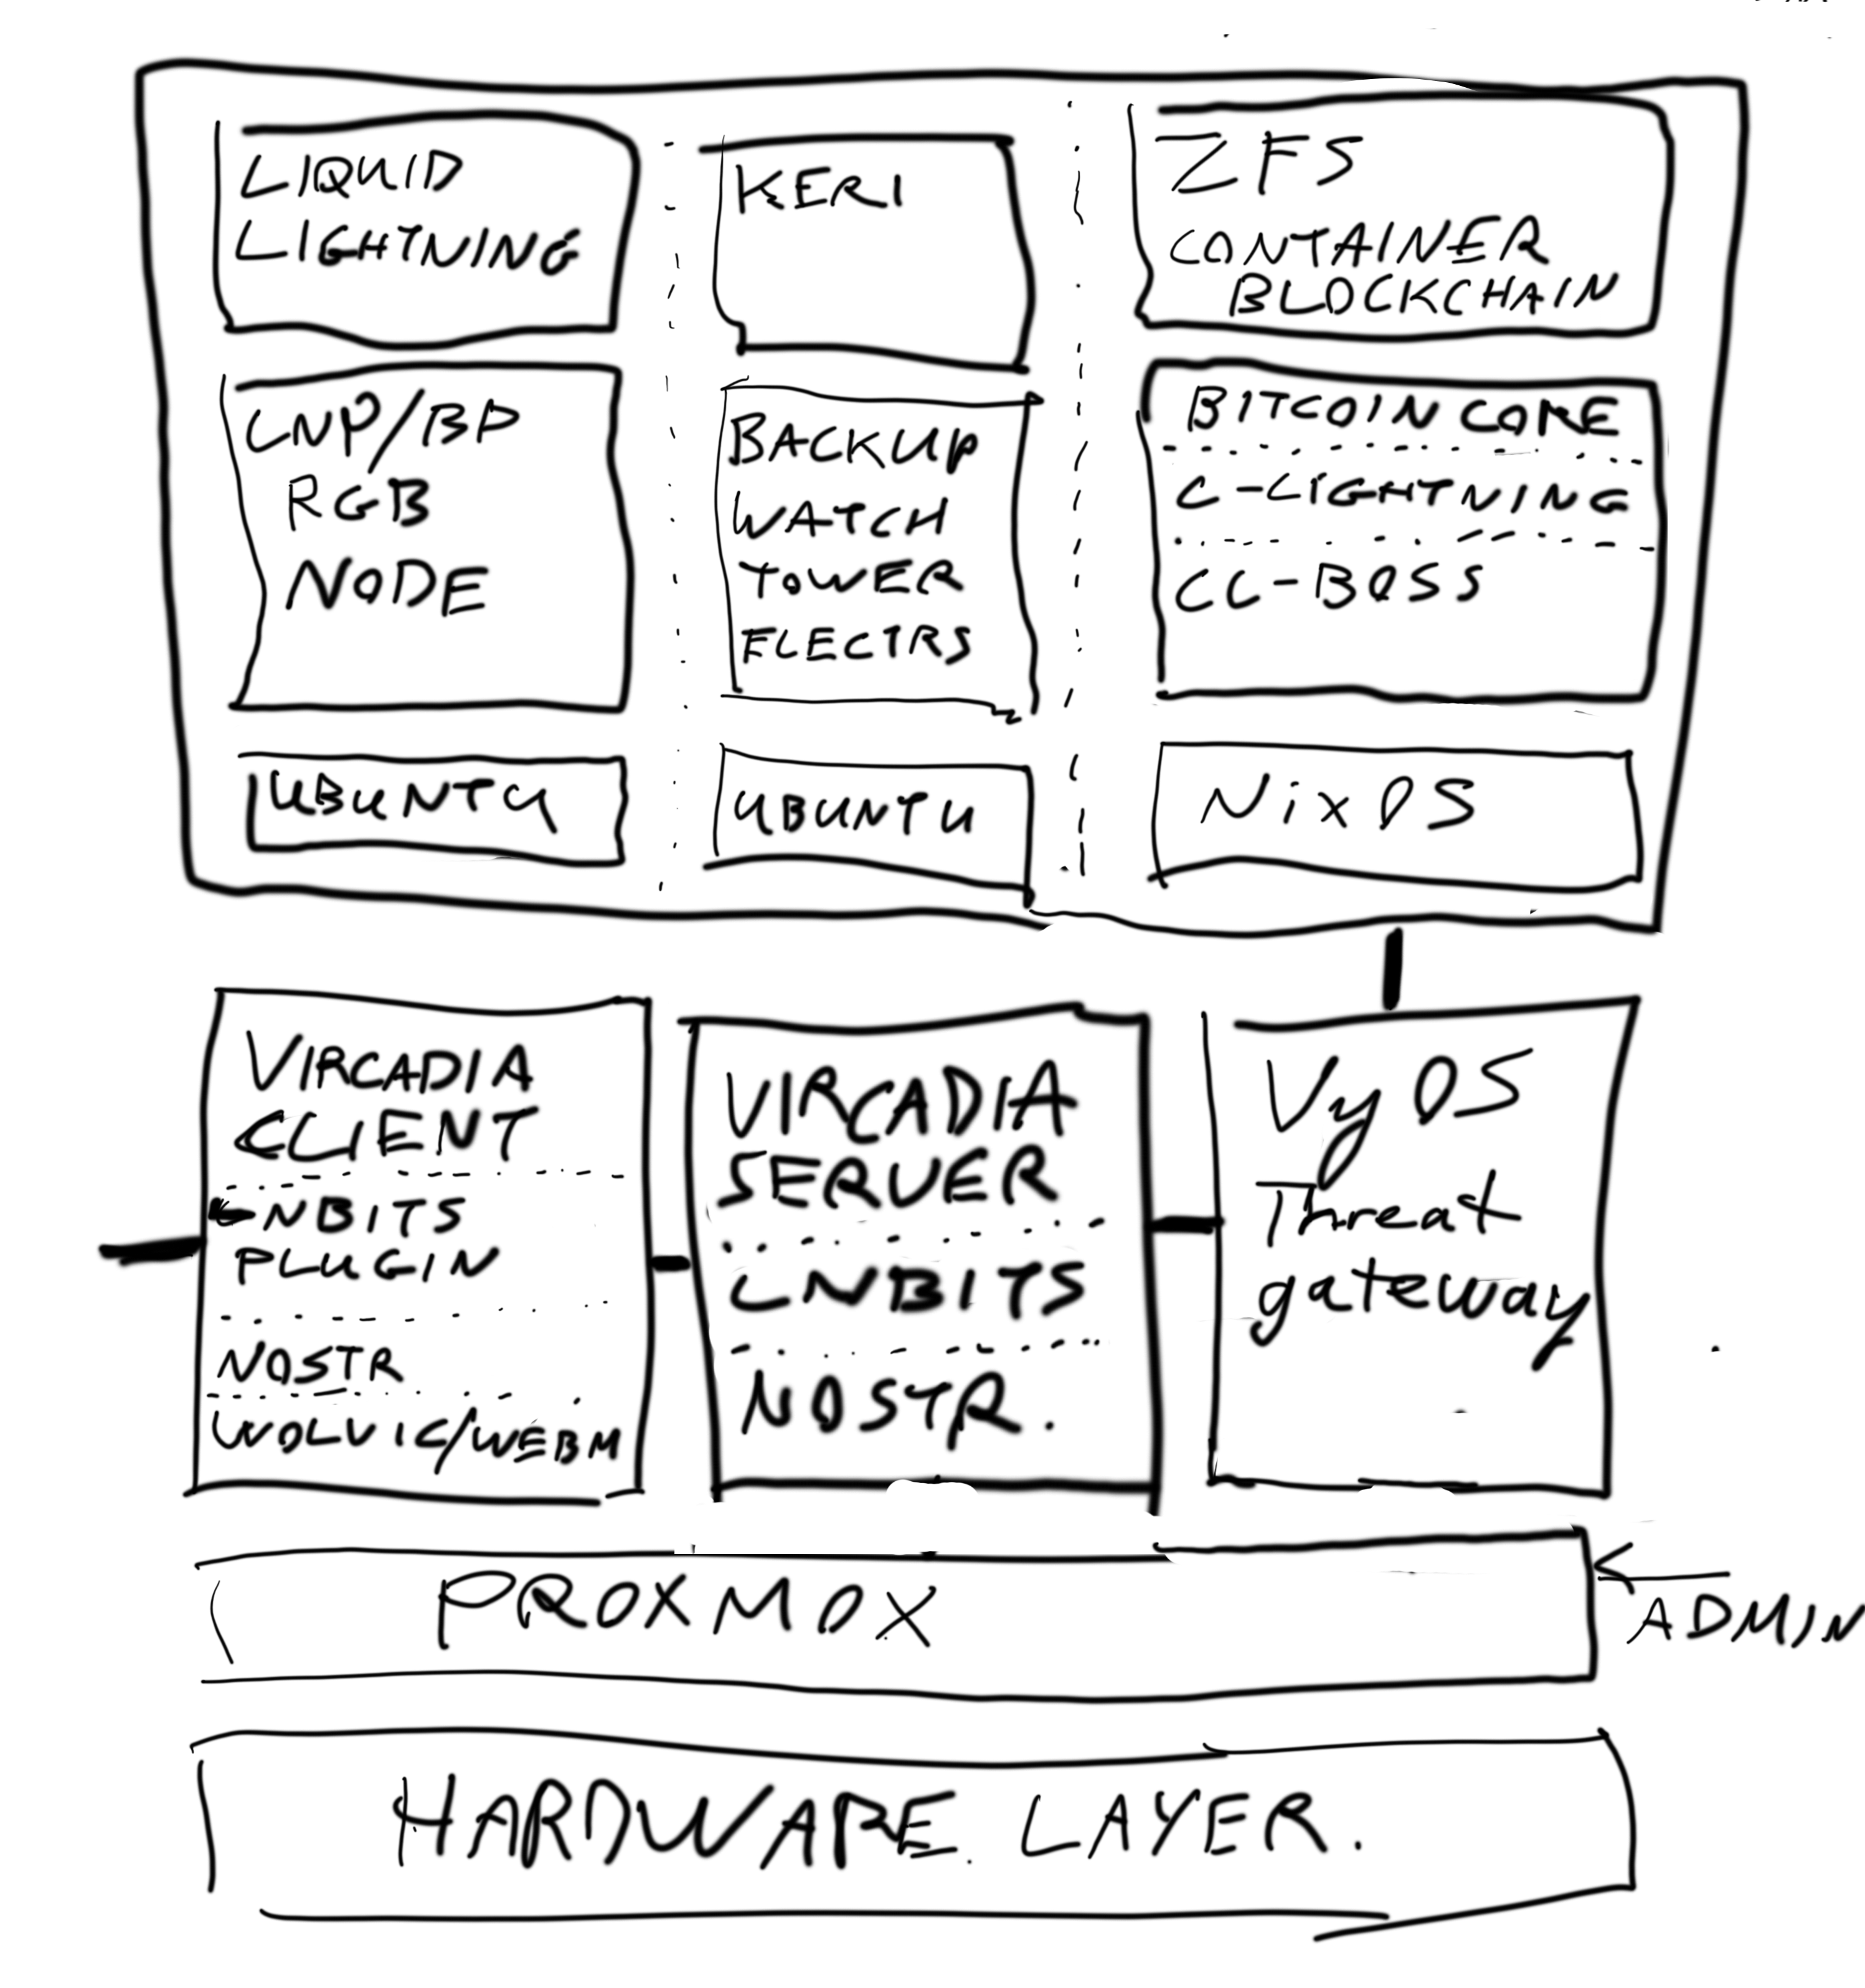
\includegraphics[width=\linewidth]{deployment}
	\caption{Proposed deployment of the software within the VMs on a single hardware system.}
	\label{fig:deployment}
\end{figure*}

\section{Networking layer}
\lipsum[50]
\subsection{Proxmox}
Proxmox open source server virtualisation allows the deployment of several virtual machines within a hardware system. Each of these VMs can have a different balance of performance, ease of use, and security. The VMs are given only the access they need to perform the task which they are specialised for. This improves overall security. Resilience is improved since elements of the cluster can be shutdown, reinstanced, and upgraded, without impacting the whole. Snapshots and backups are simplified.
\subsection{VyOS firewall}
VyOS firewall is a Proxmox aware threat management gateway and firewall which allows more nuanced interfacing with corporate systems, while maximising the security of the VM network which sits behind it i the virtual cluster.
\subsection{Privacy aspects and using TOR etc}
Currently some compromises with privacy may be necessary. Power users vs standard users. KYC/AML. 
\href{https://bitnodes.io/nodes/?q=.onion}{tor nodes}
\section{Bitcoin value management stack}
\lipsum[50]
\subsection{Bitcoin Core on NixOS}
\lipsum[50]
\subsection{Electrum server}
\href{https://blog.blockstream.com/en-esplora-and-other-alternatives-to-electrumx/}{Options on the Blockstream website}
\lipsum[50]
%\href{https://github.com/itsneski/lightning-jet}{Lightning Jet} automatic rebalance.
\subsection{C-Lightning and CLBoss}
\lipsum[50]
\subsection{LNBits with RGB and metaverse plugin}
\subsection{Backup \& Watchtower}
\lipsum[50]
\subsection{Object and media tracking: RGB}
The world database in the shared rooms in the metaverse is the global object master, with RGB client side validation inheriting and validating against these objects.\\
%Educational materials, videos, audio content and course branded objects and props are fungible tokens, authentically proved by RGB between parties. Only validated ones will be persisted in shared rooms like conferences and classes according to the room schema. Everything non compliant will be pruned. This allows educators to monetise their content, and for course participants to retain the material outside of the classroom setting where they receive them. These are fungible tokens under the RGB20 schema and can be transferred over lightning between enabled nodes. This does however imply that course participant have to run a full RGB lightning stack. This will have to be developed.\\
%NFT objects between parties like content crafted by participants (coursework, homework) are not on lightning, and will attract main chain fees. The minted material for submission will contain the nostr ID of the course participant. 
%\section{Liquid sidechain and Lightning (NFT enabled)}
%\lipsum[50]

%About Lightning Tokens: 
%https://www.youtube.com/watch?v=4k6Im5yfum0

%Detailed interview about Slashtags and %Web 3.0 aspects:
%https://twitter.com/Synonym_to/status/1481514375194292225?s=20

%Overview on all products:
%https://www.youtube.com/watch?v=5Btf_OD_3pY

%This tweetstorm is our original presentation slides:
%https://twitter.com/Synonym_to/status/1460781350441689091?s=20

%Video of the presentation:
%https://bitcointv.com/w/p1dgZcEmQQiADixvx9MoE1
\lipsum[50]
\section{Identity}
\subsection{nostr}
User authentication and sideband communication will be through nostr. This allows completely private end to end encrypted chat sessions between participants.
\section{Metaverse}
\lipsum[50]
\subsection{Vircadia}
\lipsum[50]
\subsection{Wolvic}
``The goal of the Wolvic project is to create a full-featured browser exclusively for standalone AR and VR headsets.''\\
Wolvic is a continuation of the now defunct Firefox Reality Browser project. It is open source.
\subsection{WebM}
\href{https://www.webmproject.org/about/}{Free open source web video player}	
\lipsum[50]
\section{Messengers and boards}
\subsection{Nostr}
\lipsum[50]
\subsection{Cyperpost}
\href{https://github.com/i5hi/cypherpost/}{Cyperpost} is a social platform that uses ecdsa keys for e2ee. It's private first so no plain text on servers so no scope for censorship so it's okay to be centralized. All accounts are made with a single ID pubkey derived from a social Mnemonic, so you maintain uniform ID on all platforms.
\subsection{Matrix}
Matrix is the main self hosted solution for chat and also uses ecdsa keys.
\section{Addressing identified risks}
\chapter{Example deployment }
\lipsum[50]
\section{GitHub }
\lipsum[50]